% REVISAR OS ESPACOS ENTRE O TEXTO E O PONTO FINAL!
% REVISAR OS NOMES EM INGLES, POR EXEMPLO : DESKTOP, SOFTWARE! ET COLOCAR ENG QUANDO FOR O CASO
\mainmatter
\part{Production au sein du \dsc}
\chapter{Contexte \dsc}
    \section{Qu'est-ce que \dsc ?}
    
    Le \DSC, connu sous l'acronyme \dsc, est une est une infrastructure nationale sans but lucratif pour les données de recherche en sciences humaines, axée sur les données qualitatives en Suisse, c'est-à-dire les données \eng{bitstream} telles que les images, l'audio, la vidéo et texte.
    
    La mission de \dsc est essentielle au développement d'une infrastructure de recherche numérique fiable et ouverte pour les sciences humaines en Suisse. En tant que dépositaire de données de recherche, \dsc s'engage à assurer un accès direct et durable aux données tout en permettant leur modification continue.\footnote{Voir \cite{daschmission}.} Cette mission est renforcée par l'accent mis sur l'interopérabilité et l'utilisation de normes reconnues, garantissant ainsi une intégration fluide avec les outils existants utilisés par les communautés scientifiques. De plus, l'engagement de \dsc dans la promotion des données ouvertes et dans la formation à la gestion des données de recherche témoigne de son rôle central dans l'écosystème de la recherche numérique en Suisse. Ce rôle est encore amplifié par la collaboration étroite avec les communautés de recherche, tant au niveau national qu'international, ce qui permet de maintenir une plateforme en constante évolution, adaptée aux besoins changeants des chercheurs.
    
    Les valeurs de \dsc constituent le fondement de sa mission et guident toutes ses actions. La fiabilité est au cœur de l'engagement de \dsc envers ses utilisateurs, assurant une communication transparente et le respect des délais. Cette fiabilité est complétée par une flexibilité qui permet à \dsc de répondre efficacement aux besoins spécifiques des chercheurs, en envisageant des alternatives et en proposant des scénarios adaptés. L'appréciation et la curiosité, quant à elles, favorisent un environnement de travail constructif et innovant, où les besoins des chercheurs sont constamment pris en compte et où l'exploration de nouvelles technologies est encouragée.

    Pour comprendre comment la mission et les valeurs de l'association s'alignent avec d'autres aspects, y compris sa fondation, nous allons procéder à une brève analyse de la gouvernance de \dsc.

    % logo du \dsc
    \begin{figure}[h!]
        \centering
        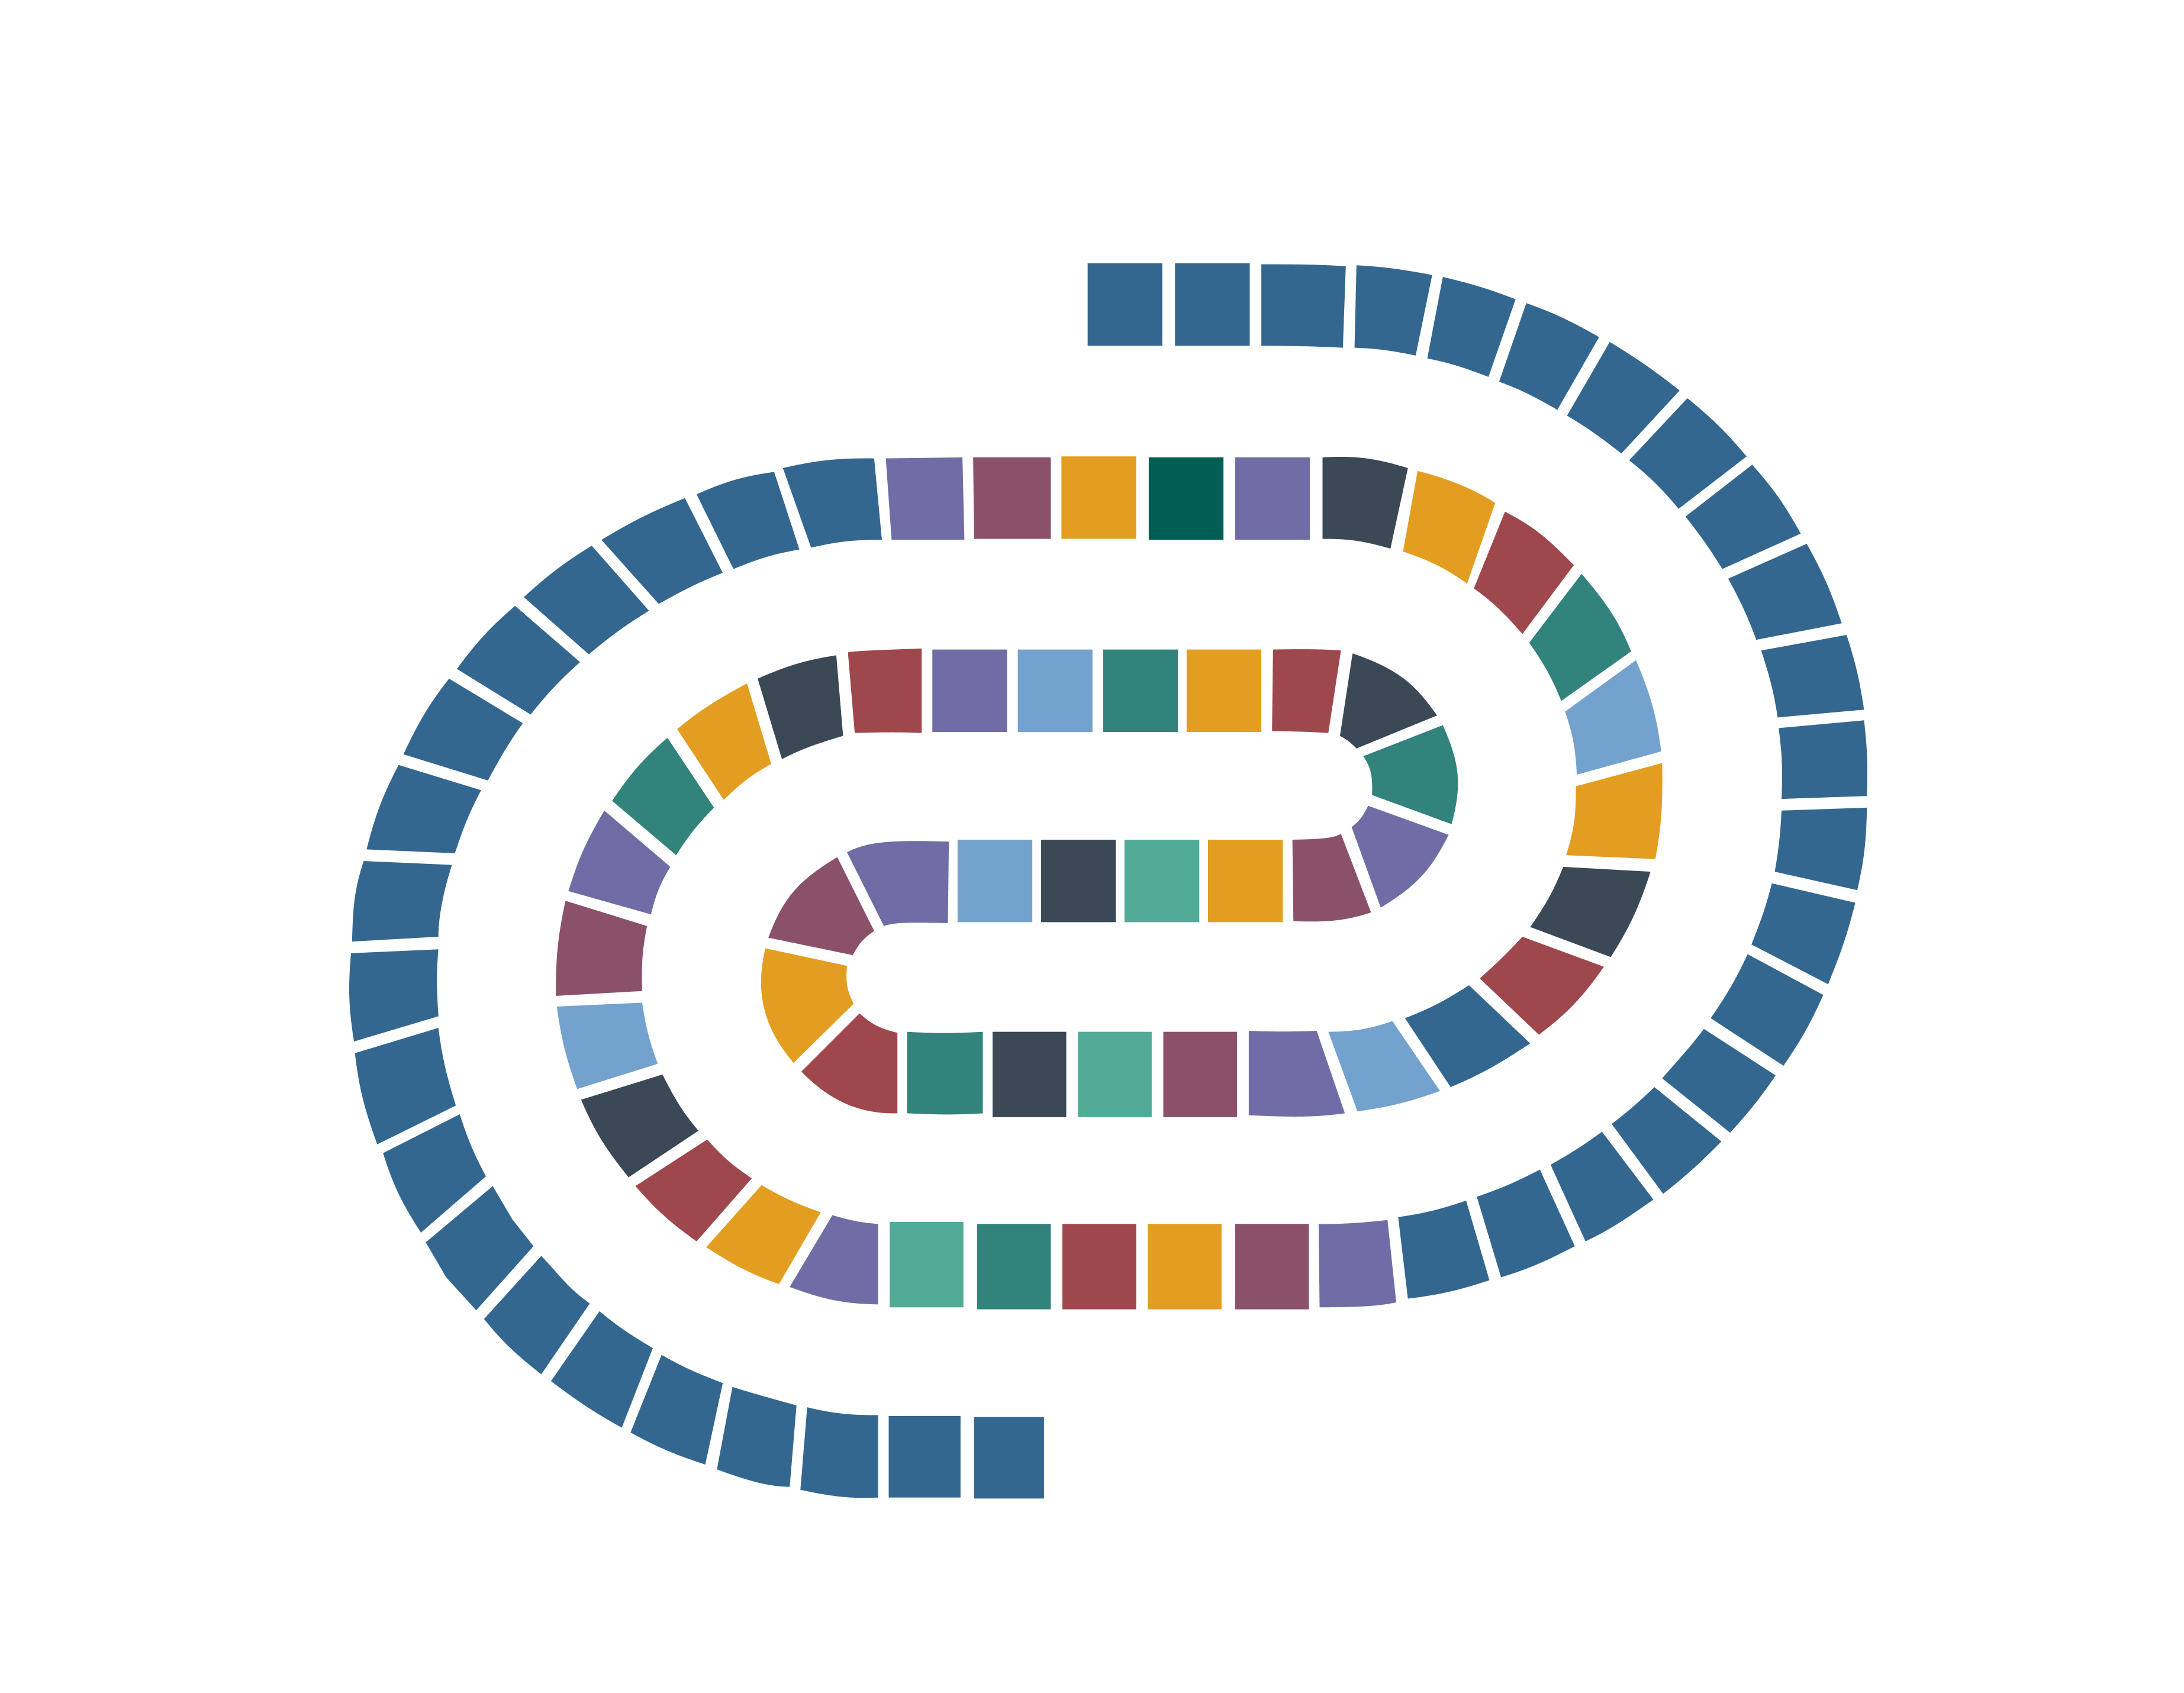
\includegraphics[width=12cm]{02_images/part_01/00_dasch_logo.png}
        \caption{Logo du \dsc}
    \end{figure}
    
        \subsection{Gouvernance du \dsc}
        
        Actuellement, l'\eng{Executive Board} du \dsc est dirigé par la Prof. Dr. \rg, qui occupe le poste de \eng{Head} du \eng{Repository Services}. Dr. Ivan Subotic est, quant à lui, le \eng{Deputy Director}. Les \eng{Repository Services}, dont Gautschy est la cheffe, englobent les départements de \eng{Product Management}, \eng{Interoperability and Archiving}. Concernant le \eng{Research Data Unit}, elle est également responsable du \eng{Research Data Management} et du \eng{Scientific Programming}. Ivan, en charge de l'\eng{Engineering}, s'occupe de l'\eng{Infrastructure}, du \eng{Software Development}, de l'\ux et du \eng{Support}.

        Par ailleurs, \rg est également l'interlocutrice principale pour d'autres partenariats du \dsc, tels que DARIAH-CH \footnote{Le consortium DARIAH-CH, constitué en novembre 2021, regroupe plusieurs institutions académiques suisses afin de favoriser la recherche et l'enseignement numériques dans le domaine des sciences humaines et sociales. Il vise à coordonner les activités liées à DARIAH en Suisse et à assurer une participation active du pays au sein de DARIAH-EU. Voir \cite{dariahch}.}, et l'\eng{Office Management}, lié à l'\unibas.

        % organigramme du \dsc
        \begin{figure}[h!]
            \centering
            \includegraphics[width=12cm]{02_images/part_01/02_executive_board.jpg}
            \caption{Organigramme du \dsc}
        \end{figure}

        % SI JAMAIS, CELA FONCTIONNE
        % \begin{figure}[htbp]
        %     \centering
        %         \savebox{\savefig}{\includegraphics[width=10cm, height=8cm]{02_images/02_executive_board.jpg}} 
        %     \rotatebox{90}{%
        %     \begin{minipage}{\wd\savefig}
        %         \usebox{\savefig}
        %         \caption{Swimlane Diagram}
        %     \end{minipage}}
        % \end{figure}

        Le \dsc adopte un modèle de gouvernance participative qui vise à englober l'ensemble des acteurs concernés par la recherche en sciences humaines en Suisse. Cette approche inclusive se traduit par une adhésion ouverte à un large éventail d'institutions, allant des universités aux académies et aux infrastructures de recherche spécialisées. Cette diversité de membres garantit une représentation équilibrée des différents domaines et perspectives de la recherche.

        Un autre aspect fondamental de la gouvernance du \dsc est son indépendance vis-à-vis de toute institution d'enseignement supérieur particulière. Cette autonomie permet d'éviter les conflits d'intérêts et d'assurer une prise de décisions objective et impartiale. En outre, l'indépendance du \dsc renforce sa crédibilité et sa légitimité en tant que plateforme neutre pour la recherche en sciences humaines.

        % gouvernance du Dasch
        \begin{figure}[h!]
            \centering
            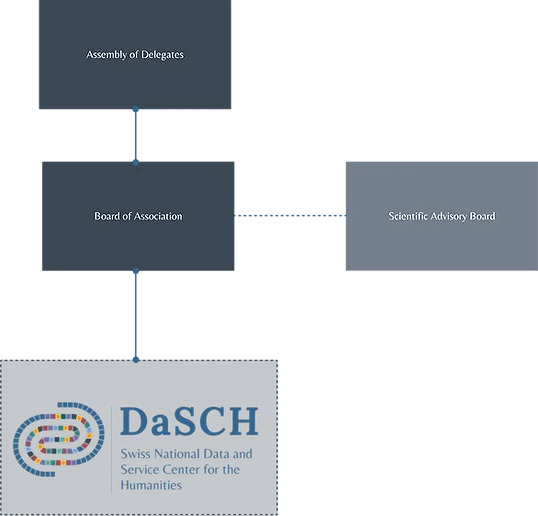
\includegraphics[width=12cm]{02_images/part_01/03_board_association.jpg}
            \caption{Gouvernance du \dsc}
        \end{figure}

        La gouvernance du \dsc est également caractérisée par son efficacité et son efficience. En limitant les formalités administratives, l'association peut se concentrer sur ses missions essentielles, telles que la mise à disposition de ressources et de services pour la recherche \footnote{Selon le site web du \dsc, l'association a \og{peu de formalités administratives}\fg. Voir \cite{gov_dasch}.}. Cette approche pragmatique permet d'optimiser l'utilisation des ressources et de garantir une réponse rapide aux besoins des chercheurs.

        La gouvernance participative et indépendante du \dsc est l'un des piliers de son fonctionnement. Pour comprendre comment cette organisation est parvenue à mettre en place une telle gouvernance efficace et inclusive, il est essentiel de revenir sur ses origines et les raisons de sa création.
    
        \subsection{Fondation du \dsc}
    
        Depuis sa création, \dsc est le fruit d'une initiative conjointe du \dhlab de l'\unibas et de la \sagw. Cette initiative a vu le jour dans le cadre d'un projet pilote ancré à \ERID 2013–2016.
    
        L'origine du \dsc remonte à un consortium réunissant les universités de Bâle, Berne et Lausanne, avec la direction assurée par le Digital Humanities Lab de l'\unibas. Ce consortium a remporté un appel d'offres public lancé par SAGW, marquant ainsi le début des efforts pour créer une infrastructure nationale dédiée aux données de recherche en sciences humaines. Pendant la phase pilote, une étude de faisabilité sur la solution technique choisie a été menée à bien, utilisant divers jeux de données.
    
        En 2017, le \dsc a été officiellement établi en tant qu'infrastructure nationale, opérée par SAGW, avec un mandat défini dans l'\erid 2017–2020. Cette reconnaissance institutionnelle a permis au \dsc de se structurer et de s'intégrer pleinement dans le paysage national de la recherche en sciences humaines, en apportant des solutions innovantes pour la gestion et la préservation des données de recherche.
        
        Depuis 2021, le \dsc fonctionne comme une infrastructure nationale de données de recherche, bénéficiant principalement d'un financement de la part du \SNSFn. Cette évolution témoigne de l'importance croissante des humanités numériques et de la reconnaissance de la nécessité de disposer de structures robustes et durables pour le archivage, l'accès et l'exploitation des données de recherche dans ce domaine.

        
        \begin{figure}[h!]
            \centering
            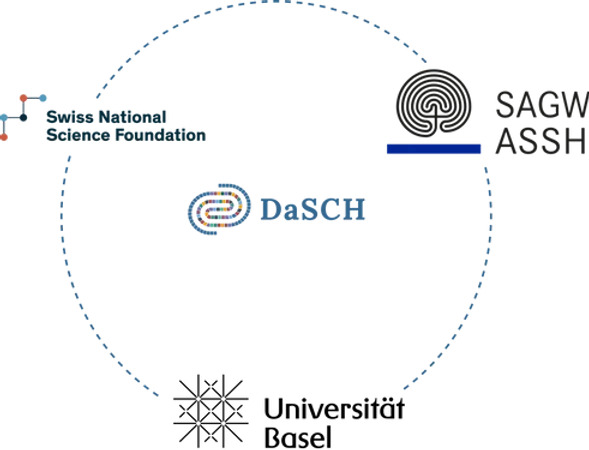
\includegraphics[width=12cm]{02_images/part_01/01_funding.jpg}
            \caption{Schéma de fonctionnement du \dsc}
        \end{figure}
    
        Ainsi, la fondation du \dsc illustre une réponse concertée aux besoins émergents des sciences humaines à l'ère du numérique, en mettant en place des infrastructures capables de soutenir les chercheurs dans leurs travaux et de valoriser les données produites par leurs recherches. Fort de ce socle, le \dsc a mis également en place une plateforme numérique qui va bien au-delà du simple archivage de données. Nous allons donc aborder par la suite comment fonctionne cette plateforme.

        
        \subsection{\dsc et l'\opdt en Suisse}

        \dsc possède une plateforme pour les données de recherche ouvertes dans les sciences humaines en Suisse. Cet environnement de recherche virtuel peut être utilisé tant pour ceux et celles qui veulent publier ces données quant pour ceux et celles qui veulent réutiliser ses données \footnote{Voir \cite{re3data}.}. C'est aussi important souligner que \dsc développe et exploite un dépôt à long terme conforme aux principes FAIR (\eng{Findable}, \eng{Accessible}, \eng{Interoperable}, \eng{Reusable}). Pour ces raison, nous pouvons voir que \dsc s’assure que les informations collectées soient non seulement accessibles et réutilisables par la communauté scientifique, mais aussi qu’elles respectent les normes internationales de gestion de données. Cela permet non seulement de préserver le patrimoine scientifique de manière durable, mais aussi de faciliter la collaboration et l’innovation au sein de la communauté académique.

        En deuxième place, l’environnement de recherche virtuel proposé par \dsc offre aux chercheurs une plateforme intégrée qui simplifie l’archivage, la gestion et le partage de leurs données. Cette infrastructure est essentielle pour promouvoir la transparence et l’efficacité dans les processus de recherche, en assurant que les données sont disponibles et exploitables à long terme. Cela va de soi avec l'idée de \psdn, une fois que ce processus d'archivage permet une identification de données.

        Néanmoins, l'archivage de données en soi n'assure pas une \psdn lors de l'interopérabilité. Pour montrer comment ces données sont interprétées et comprises, ainsi que la manière dont la communauté est intégrée, nous allons maintenant analyser les stratégies de \dsc.
        
        \subsection{Stratégies de \dsc}
        La stratégie de \dsc repose sur trois piliers fondamentaux, chacun jouant un rôle essentiel dans la réalisation de ses objectifs à court et long terme \footnote{Les trois pilliers mentionnés sont expliqués dans la partie \eng{Strategic Goals} sur le site. Voir \cite{daschstrategicgoals}.}. Le premier pilier, l'extension technique de la plateforme, est une réponse directe aux besoins croissants d'évolutivité et de flexibilité dans la gestion des données de recherche. En rendant la plateforme plus accessible et adaptable, \dsc vise à offrir aux chercheurs un outil performant et intuitif, tout en permettant l'intégration de nouvelles technologies. Cela ne se limite pas à l'amélioration de l'expérience utilisateur, mais s'étend également à l'augmentation de l'interopérabilité en encourageant l'adoption de standards reconnus et de données normées. Cette approche permet non seulement de faciliter la réutilisation des données, mais aussi d'assurer leur pérennité dans un environnement de recherche en constante évolution.
        
        Le deuxième pilier de la stratégie de \dsc est le soutien à la création de communauté et à l'éducation. \dsc reconnaît que la technologie seule ne suffit pas à garantir le succès de sa plateforme. En connectant les chercheurs entre eux et en leur offrant des opportunités de formation, \dsc renforce les liens au sein de la communauté scientifique. Cela inclut non seulement l'organisation d'événements pour échanger sur les besoins et les défis rencontrés, mais aussi l'offre de formations adaptées, en particulier pour les jeunes chercheurs. Cette orientation vers l'éducation et le soutien communautaire est cruciale pour garantir que la plateforme \dsc soit non seulement utilisée, mais aussi optimisée et améliorée grâce aux retours de ses utilisateurs, assurant ainsi une évolution en phase avec les besoins réels des chercheurs.
        
        Enfin, le troisième pilier consiste en un renforcement des réseaux et des coopérations, tant au niveau national qu'international. \dsc comprend que la collaboration est essentielle pour avancer dans la recherche et la gestion des données. En s'associant avec d'autres institutions et en participant activement à des projets internationaux, \dsc vise à créer des synergies qui permettent de développer des solutions innovantes pour l'accessibilité, l'interopérabilité et la conservation à long terme des données. L'engagement de \dsc dans des initiatives comme DARIAH et la définition de standards IIIF pour les images 3D témoigne de sa volonté de jouer un rôle de premier plan dans la normalisation et l'amélioration des pratiques de gestion des données de recherche. Cette stratégie de coopération est non seulement bénéfique pour \dsc, mais elle contribue également à l'avancement de la recherche en sciences humaines dans son ensemble.

        Le développement et le maintien d'une infrastructure et des stratégies aussi complexe que \dsc nécessitent des investissements conséquents et durables. Nous allons expliquer alors comment s'opère le financement de l'association.
        
        \subsection{Financement du \dsc}

        Concernant le financement du \dsc, l'association bénéficie d'un financement principal du SNSF, qui a octroyé un soutien significatif pour la période 2021 à 2024, intitulé \erid 2021-2024. Cet accord de financement a permis de définir clairement les services que le \dsc doit fournir à la communauté scientifique suisse. En plus de ce financement public, l'\unibas apporte des contributions en nature, telles que l'hébergement de l'infrastructure et la mise à disposition de ressources humaines.

        Ces ressources financières permettent au \dsc de développer et de maintenir une infrastructure numérique. Cependant, pour étendre ses services et répondre à des demandes spécifiques, le \dsc peut également solliciter des financements supplémentaires auprès de tiers ou des utilisateurs eux-mêmes. Ces contributions peuvent prendre la forme de partenariats, de projets de recherche ou de frais d'utilisation de certains services.

        Nous allons maintenant nous pencher plus en détail sur l'\erid pour comprendre comment il fonctionne et pourquoi il est important pour comprendre les enjeux du \dsc dans ce contexte de \psdn.

            \subsubsection{Fonctionnement de l'\erid}
            Le système politique fédéral suisse considère que les investissements dans l'éducation, la recherche et l'innovation sont essentiels pour le succès du pays. C'est pourquoi des investissements sont réalisés dans ces domaines, car il est estimé que l'éducation et la recherche sont les fondements de la créativité et de l'entrepreneuriat. Ces éléments sont également des prérequis pour la capacité d'innovation et la compétitivité des entreprises suisses. Afin de soutenir les initiatives dans ces trois domaines, la Confédération suisse et les cantons financent et régulent le secteur de l'ERI par le biais du plan \ERID, accordé tous les quatre ans, afin de promouvoir ces initiatives \footnote{Le caractère cyclique des évaluations ERI peut conduire à des fluctuations dans l'importance accordée aux indicateurs DaSCH, ce qui peut créer une certaine instabilité dans les politiques publiques associées.}.
    
            Il est important de noter que le plan \erid est soumis à l'Assemblée fédérale avant d'être approuvé. Pour la période 2021-2024, à laquelle \dsc est associé, un investissement de 28,1 milliards de \textsc{chf} a été prévu, soit plus de 2 millions de \textsc{chf} par rapport au plan \ERID 2017-2020, qui est à l'origine de \dsc\footnote{Voir \cite{sbfi}.}.

            \begin{figure}[h!]
                \centering
                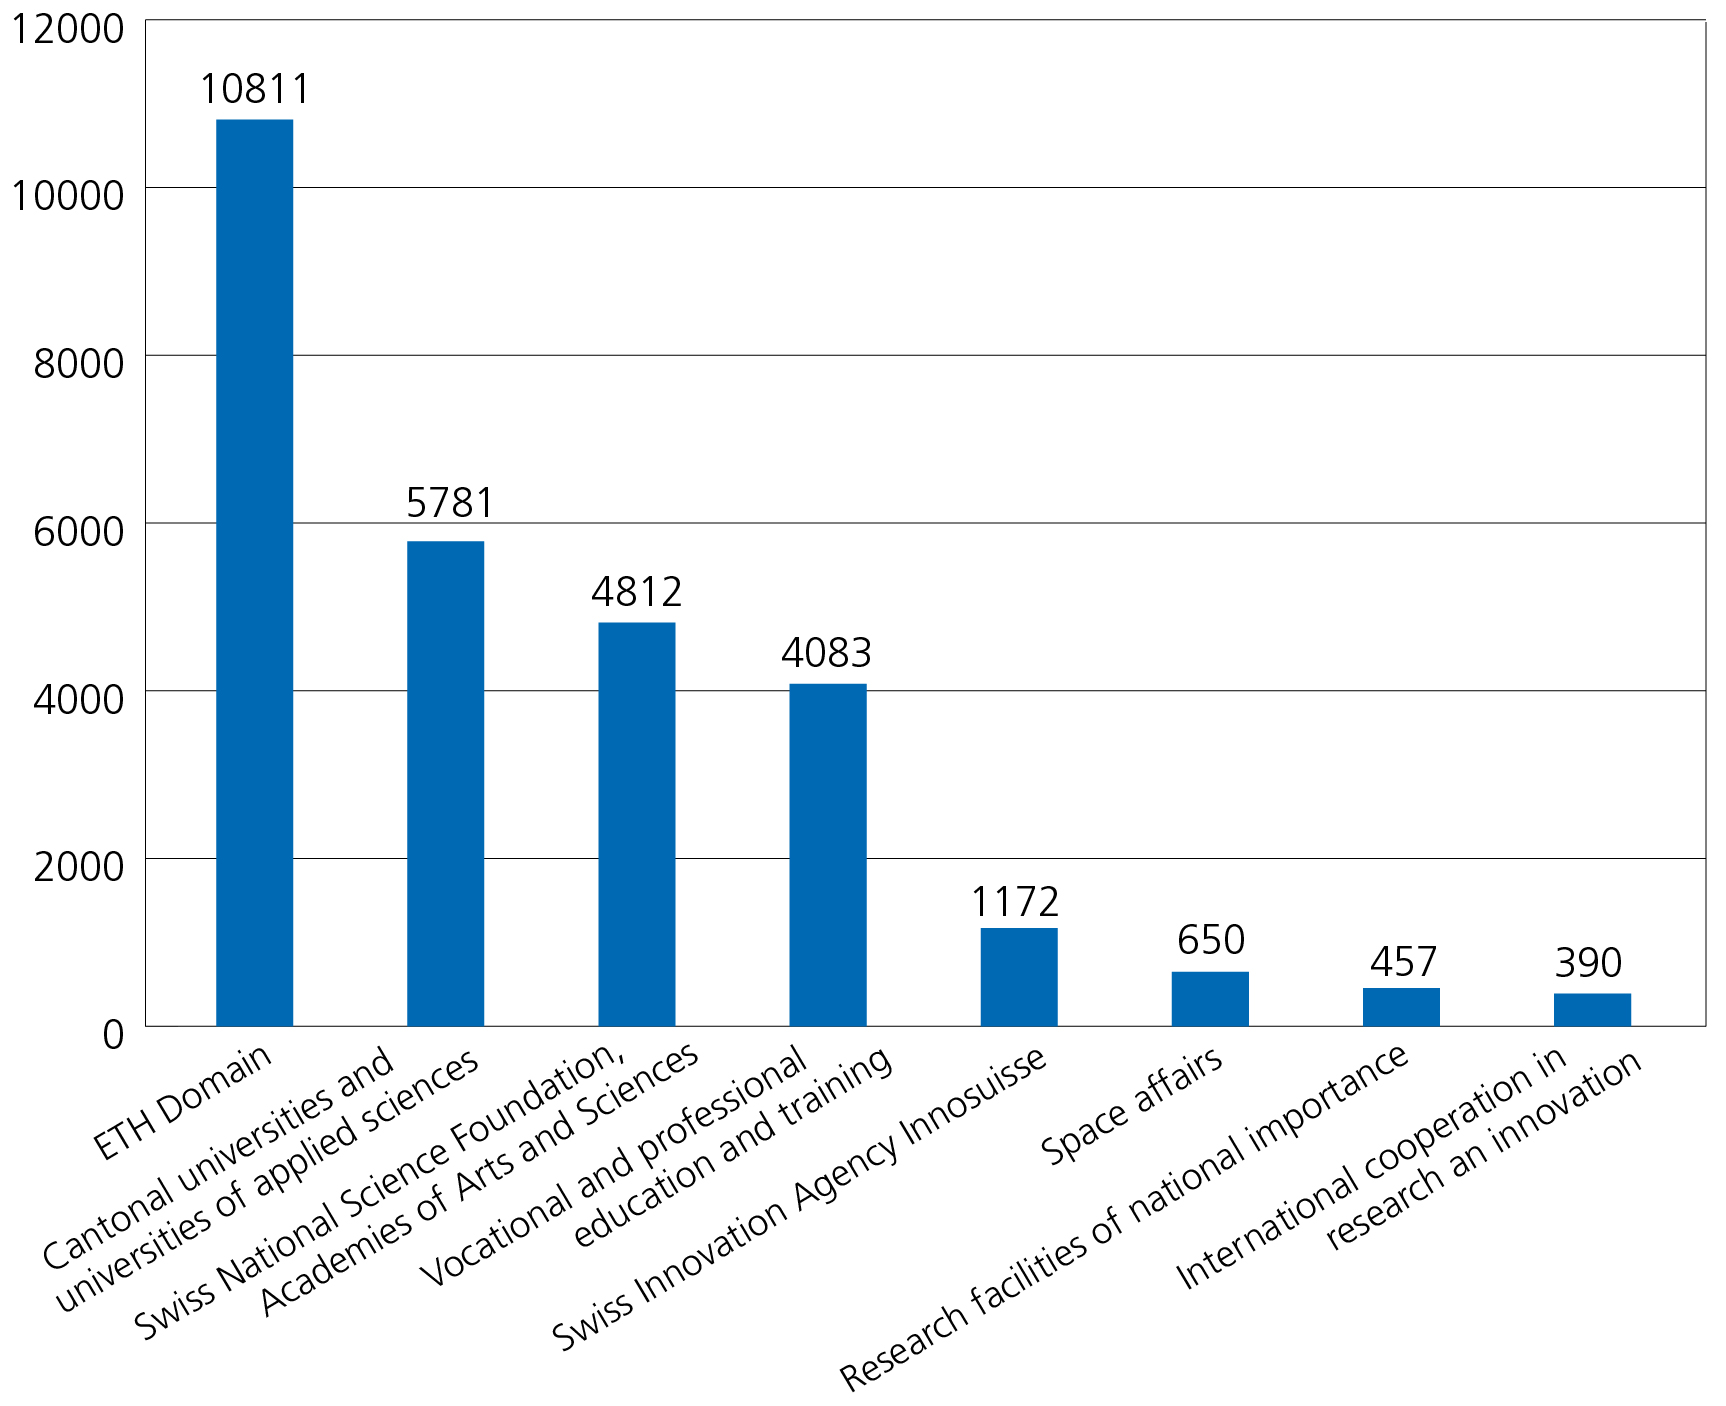
\includegraphics[width=12cm]{02_images/part_01/04_investissemnt_eri_2021_2024.jpg}
                \caption{Financement \erid alloué par l'Assemblée fédérale suisse pour 2021-2024, en millions. \textbf{Source} : \cite{sbfi}.}
            \end{figure}
    
            Enfin, il est également crucial de souligner que pour la période 2021-2024, les politiques du plan \ERID se concentrent sur trois thèmes principaux : la numérisation, le développement durable et l'égalité des chances. Ces politiques bénéficient de l'engagement des cantons et de tous les parties prenantes concernées\footnote{Voir \cite{sbfi}.}.

        
        \subsection{Notes conclusives}
        
        En conclusion, \dsc joue un rôle crucial dans la transformation numérique des sciences humaines en Suisse, en fournissant les outils et les services nécessaires pour une gestion optimale des données de recherche ouvertes, tout en respectant les plus hauts standards de qualité et de durabilité. Nous avons également constaté que pour \dsc, le standard IIIF occupe une place centrale dans ses préoccupations en matière de maintien de la persistance des données. C'est pourquoi nous allons maintenant nous pencher sur ce qu'est le standard IIIF, afin de comprendre l'importance qu'il a revêtue lors de la mise en œuvre des \eng{pipelines} au cours de mon stage.


\chapter{Contexte IIIF}

    \section{Qu'est-ce que l'IIIF ?}
    
    Le standard \iiif est un ensemble de normes ouvertes conçues pour la gestion des objets numériques. Soutenues par une communauté internationale, les APIs IIIF constituent un élément fondamental en permettant l'ajout d'informations descriptives aux objets numériques. Cela assure non seulement que ces informations soient accessibles et compréhensibles pour les utilisateurs humains (\textit{human readable}), mais facilite également l'affichage des images. De plus, la communauté IIIF s'efforce constamment de maintenir et d'améliorer ces APIs, garantissant ainsi leur compatibilité avec une large variété d'objets 2D. De plus, avec l'introduction de la version 4.0, des discussions sont en cours pour étendre ce support aux modèles 3D, ouvrant ainsi de nouvelles perspectives dans la gestion des ressources numériques.
    
    Avant de nous plonger plus profondément dans les aspects techniques de l'API 3.0, il est pertinent de comprendre l'histoire de son développement, ce qui nous permet de mieux saisir les enjeux actuels et les futures évolutions envisagées par la communauté.

    \section{Origines d'IIIF}
    
    L'origine d'IIIF daterait environ du début des années 2010, à partir d'une discussion informelle entre technologistes de \eng{Stanford University}, \eng{Oxford University} et de la \eng{British Library} dans un café, et, par la suite, différentes bibliothèques nationales et internationales ont rejoint l'initiative \footnote{Les deux versions sont d'accord sur les années du début, néanmoins c'est la thèse de Raemy qui raconte qui étaient les acteurs principaux et les institutions lors de la création d'IIIF. Pour les deux versions, voir la thèse de Raemy \cite[p.~13]{raemy2017iiif} et le site de Biblissima, Voir \cite{biblissima_iiif_intro}}. IIIF est actuellement un \textit{consortium} international qui rassemble différentes organisations du monde et qui a également une communauté de musées, archives, bibliothèques, instituts de recherche, sociétés de services informatiques qui entretiennent les APIs IIIF.

    La communauté IIIF a pour mission de définir, de diffuser et de faire évoluer les normes techniques IIIF en s'appuyant sur des cas d'usage concrets. C'est dans cette perspective que l'ambition de IIIF est de créer un cadre technique commun, permettant aux fournisseurs de ressources numériques de délivrer leurs contenus de manière standardisée sur le Web, afin de les rendre consultables, manipulables et annotables par n'importe quel logiciel compatible \footnote{Voir \cite{biblissima_iiif_intro}}.

    % schéma IIIF
        \begin{figure}[h!]
            \centering
            \includegraphics[width=12cm]{02_images/part_01/09_schema_iiif.png}
            \caption{Schéma : principe général d’interopérabilité de IIIF (trois applications différentes sont branchées à trois entrepôts IIIF).}
        \end{figure}
     
    \section{Intégration d'IIIF pour la valorisation du patrimoine}
    
    Le standard IIIF (International Image Interoperability Framework) s'est imposé comme un outil incontournable pour l'archivage et la diffusion d'objets numériques au sein des institutions patrimoniales. En associant un objet numérique à un fichier \textsc{json}, ce standard offre une méthode simple et flexible pour décrire et rendre accessible un large éventail de ressources.

    Dans un premier temps, il est essentiel de souligner l'adoption généralisée du IIIF par de nombreuses institutions culturelles de renommée mondiale, telles que la Bibliothèque nationale de France ou les Musées du Vatican. Cette adhésion massive témoigne de l'efficacité du standard pour répondre aux besoins spécifiques des institutions patrimoniales, en particulier en matière de préservation et de valorisation des collections.
    
    Ensuite, la popularité du IIIF s'explique par sa capacité à rendre les objets numériques et leurs métadonnées accessibles à un large public grâce à des \eng{viewers} en ligne, qui sont des outils pour rendre les modèles 3D visibles sur le web, tels Mirador, Universal Viewer et OpenSeadragon \footnote{Mirador, Universal et OpenSeadragon sont trois projects \opso qui permettent de visualiser ces modèles 3D. Pour plus de détails sur ces viewers, Voir \cite{mirador}, \cite{universalviewer} et \cite{openseadragon}}. Ces outils permettent également d'explorer les collections de manière interactive, de réaliser des comparaisons, d'annoter les images et voire de zoomer en haute définition \footnote{Alors que le texte de Rossenova vise un large public, il faut souligner que les \eng{viewers} permettent ces autres possibilités. Voir \cite{rossenova2023iiif}.}. Cette dimension visuelle est particulièrement appréciée des chercheurs et du grand public, qui peuvent ainsi bénéficier d'une expérience utilisateur enrichie. Voyons un exemple avec Mirador \footnote{Pour regarder la démonstration de Mirador, Voir \cite{mirador_demo}.} :

    % Mirador : comparaison
        \begin{figure}[h!]
            \centering
            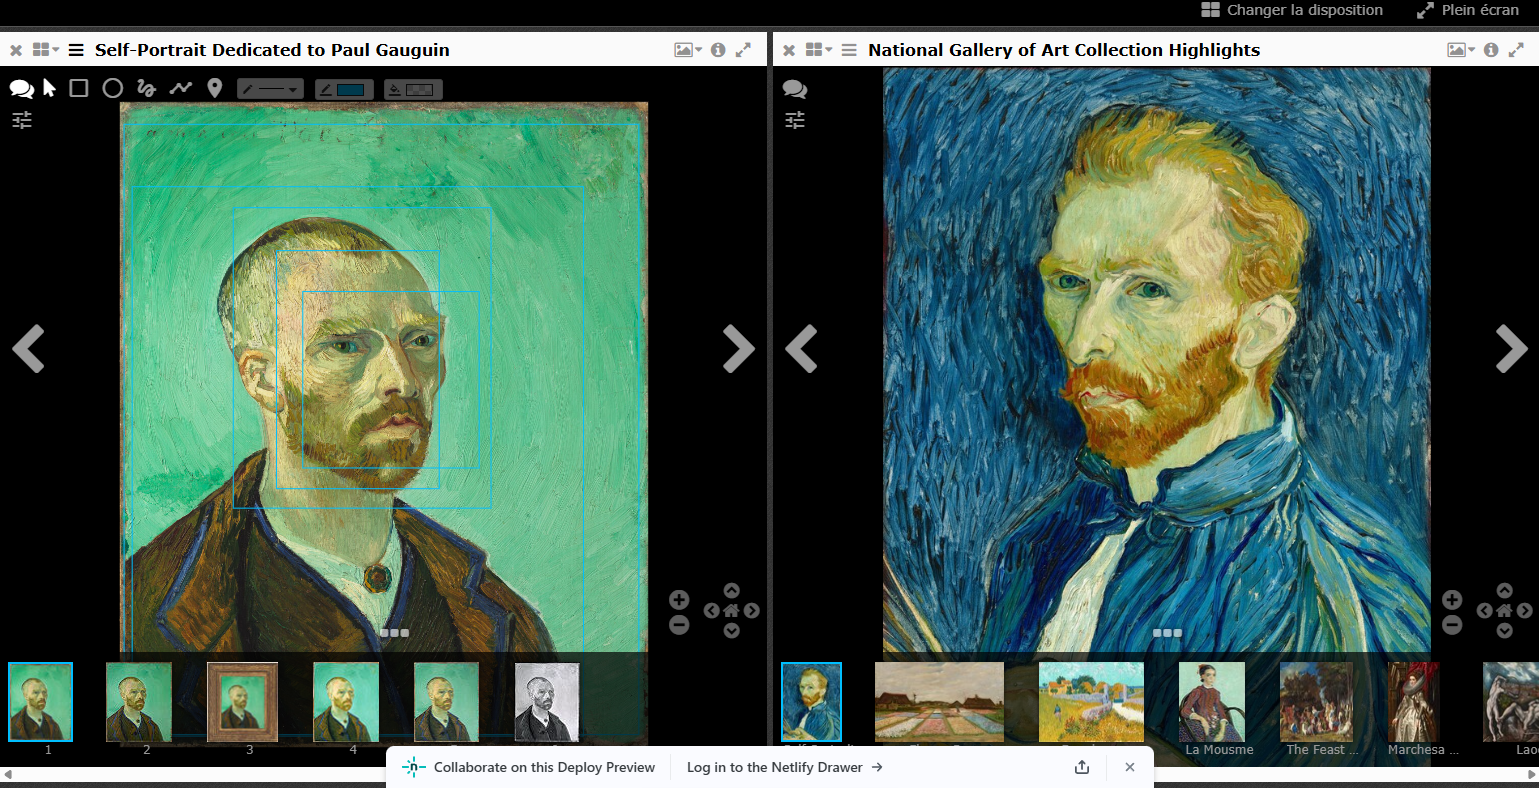
\includegraphics[width=12cm]{02_images/part_01/11_mirador_01.png}
            \caption{Mirador: comparaison entre images de différentes institutions.}
        \end{figure}

    % Mirador : exemple d'annotation
        \begin{figure}[h!]
            \centering
            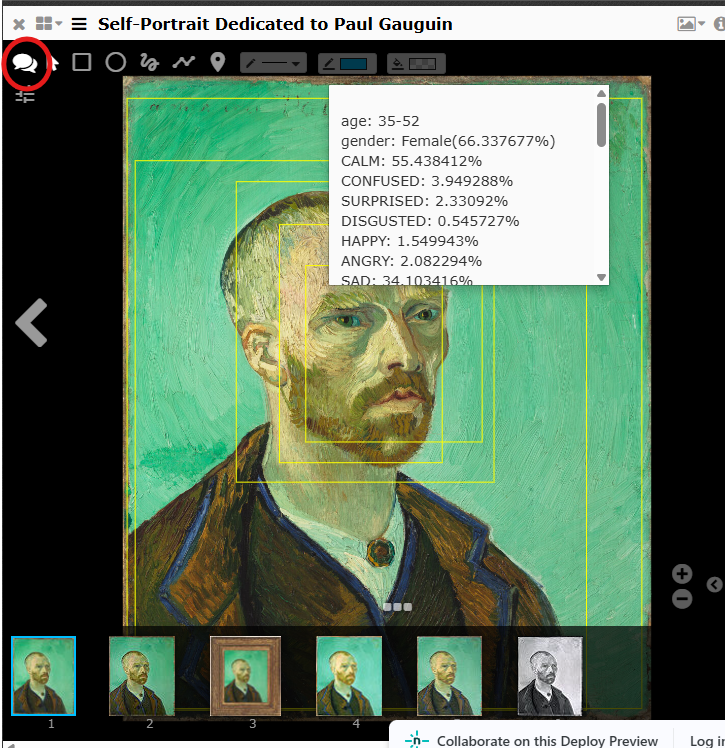
\includegraphics[width=12cm]{02_images/part_01/12_mirador_02.png}
            \caption{Mirador: exemple d'image annotée, avec l'outil d'annotations du \eng{viewer}.}
        \end{figure}

    % Mirador : zoom en haute définition de l'image de Van Gogh
        \begin{figure}[h!]
            \centering
            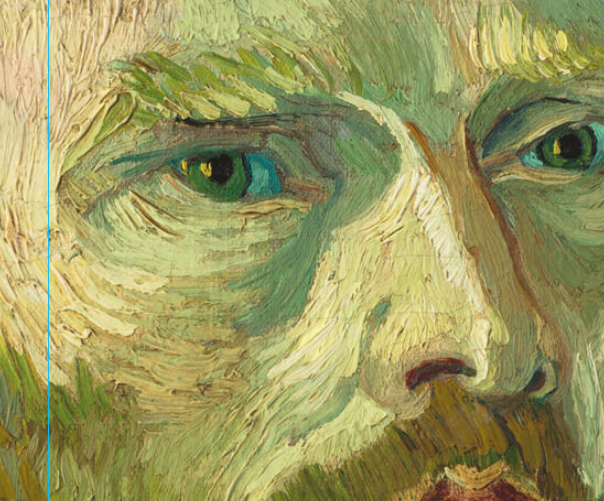
\includegraphics[width=12cm]{02_images/part_01/13_mirador_03.png}
            \caption{Mirador : zoom en haute définition dans un détail de la première image.}
        \end{figure}
    
    Par ailleurs, le IIIF offre une grande flexibilité dans la structuration des données. Il est ainsi possible d'archiver des objets avec un minimum d'informations, ce qui facilite l'intégration rapide de nouvelles acquisitions dans les collections. De plus, le standard permet de décrire des objets complexes et de gérer des ensembles d'images multiples, favorisant ainsi une approche holistique de l'archivage.
    
    En outre, le IIIF joue un rôle essentiel dans la diffusion d'images haute résolution. En réduisant les contraintes liées au stockage et à la bande passante, il permet de partager des images de grande qualité sans compromettre les performances. Cette caractéristique est particulièrement intéressante pour les institutions qui souhaitent mettre à disposition du public des reproductions numériques de haute fidélité de leurs œuvres.
    
    Enfin, l'une des forces du IIIF réside dans sa capacité à favoriser l'interopérabilité entre les différentes institutions. Grâce aux manifestes IIIF, il est possible de créer des liens entre des objets provenant de sources diverses et de construire des narrations entre eux. Cette fonctionnalité ouvre de nouvelles perspectives pour la recherche et la collaboration entre les institutions culturelles.
    
    En conclusion, le standard IIIF constitue une solution efficace et flexible pour l'archivage et la diffusion d'objets numériques. En offrant une structure simple et ouverte, il permet aux institutions patrimoniales de préserver leur patrimoine et de le rendre accessible à un public toujours plus large. Cependant, l'exploitation optimale du IIIF nécessite une réflexion approfondie sur les enjeux liés à la gestion des données, à l'interopérabilité et à la pérennité des infrastructures numériques.

    \section{IIIF API 3.0.}
    
    L'importance d'expliquer l'API 3.0 réside dans le fait qu'elle est la plus utilisée par les institutions travaillant dans le domaine patrimonial. De plus, elle constitue la base pour la conception de l'API 4.0. Il est donc fondamental de bien comprendre les principes de l'API 3.0 pour saisir non seulement son importance actuelle, mais aussi les raisons pour lesquelles elle a été essentielle dans le cadre de mon stage.
    
    L'API IIIF 3.0 se compose de quatre API RESTful au format JSON-LD : Image API, Presentation API, Content Search API et Authentification API. Pour bien comprendre chacune de ces API dans notre étude, nous allons en expliquer le fonctionnement et analyser ensuite les enjeux pour \dsc avec les applications développées durant le stage, ce qui nous aidera à comprendre l'importance future de l'API 4.0 pour notre travail.
    

    \subsubsection{Image API}
    
    La première version de l'\iapit a été lancée en août 2012 \footnote{Voir Pour ces prochains chapitres, nous avons suivi l'ordre chronologique explicatif suggéré par les travaux de Julien Raemy. Voir \cite{raemy2017iiif}} et la fonction basique de cette API est de prendre les données techniques d'une image et ses informations associées, pour les rendre visibles sur le web \footnote{Tous les concepts du chapitre ont été extraits et analysés à partir de la partie dédiee au \iapit sur le site d'IIIF. Voir \cite{iiifimage30}.}. Pour ce faire, elle requiert une URI définie selon une syntaxe stricte (Voir Tableau 2.1) \footnote{L'exemple de syntaxe a été extrait de la section d'Image API sur le site d'IIIF. Voir \cite{iiifimage30} En ce qui concerne l'idée de faire un tableau avec les requêtes, ce travail s'est inspiré de la suggestion de Raemy. Voir \cite[p.~20]{raemy2017iiif}.}.
    
        \begin{table}[h!]
        \centering
        \caption{Structure des requêtes d'image et d'information}
        \resizebox{\textwidth}{!}{
                \begin{tabular}{|l|l|}
                \hline
                \rowcolor{gray!20} % première ligne grise
                \textbf{Type de Requête}        & \textbf{Structure de la Requête}                                                                                      \\ \hline
                \textbf{Image Request}          & \{scheme\}://\{server\}\{/prefix\}/\{identifier\}/\{region\}/\{size\}/\{rotation\}/\{quality\}.\{format\}              \\ \hline
                \textbf{Exemple Image Request}  & \texttt{http://www.example.org/image-service/abcd1234/full/full/0/default.jpg}                                       \\ \hline
                \textbf{Image Information Request} & \{scheme\}://\{server\}\{/prefix\}/\{identifier\}/info.json                                                        \\ \hline
                \textbf{Exemple Information Request} & \texttt{http://www.example.org/image-service/abcd1234/info.json}                                                   \\ \hline
                \end{tabular}
            }
        \end{table}

    
    Comme nous pouvons le constater, les informations sont prises dans l'ordre indiqué dans le tableau. Il est important de mentionner que l'API ne pose aucune restriction quant à la forme des identifiants qu'un serveur peut utiliser ou prendre en charge, ce qui offre une grande flexibilité, même dans la conception des identifiants.
    
    L'image renvoyée est toujours la représentation de l'URI, ce qui signifie que l'URI peut modifier la nature de l'image affichée. Cela est crucial pour certaines institutions, car des paramètres comme la taille en \eng{pixels}, la couleur, ou d'autres aspects peuvent être ajustés en fonction des besoins spécifiques.
    
    \subsubsection{Presentation API}
    
    Le \eng{Presentation API} travaille avec des objets numérisés ou nativement numériques et son objectif principal est de fournir les informations nécessaires pour permettre une visualisation riche en ligne des objets numériques composés, souvent en combinaison avec l'\iapit \footnote{Tous les concepts du chapitre ont été extraits et analysés à partir de la partie dédiée au \papit sur le site d'IIIF. Les sources seront citées à chaque fois que cela sera nécessaire pour garantir la clarté sur les références. Voir \cite{iiifpresentation30}.}. Ces objets sont standardisés suivant une description en format \textsc{json}. Un objet dit composé peut être une série de pages, de surfaces, etc. Par exemple, il peut s'agir des deux faces d'une photographie, des quatre vues cardinales d'une statue, de papyrus, etc. Toutes ces spécifications suivent les principes du Linked Data et de l'architecture du Web pour garantir leur interopérabilité. De plus, le modèle de données Shared Canvas et \textsc{json-ld} permet de créer un format \textsc{json} facile à mettre en œuvre.
    
    Pour bien comprendre le fonctionnement du \eng{Presentation API} d'IIIF, il est essentiel de savoir comment les types de ressources sont classés dans la spécification des objets composés. Le modèle est structuré de la manière suivante : Collection, Manifest, Canvas et Range \footnote{Voir \cite{iiifpresentation30}}.
    
    Premièrement, une Collection est une liste ordonnée de Manifests et/ou d'autres Collections. Les Collections permettent de regrouper des Manifests et d'autres Collections dans une structure hiérarchique pour la présentation. Cette présentation peut être utilisée pour naviguer, afficher des résultats de recherche dynamiques ou fournir un ensemble de ressources fixes, quel que soit l'objectif \footnote{Voir \cite{iiifpresentation30}}.
    
    Deuxièmement, le Manifest décrit la structure et les propriétés d'un objet composé. Il contient les informations nécessaires pour qu'un client puisse afficher le contenu à un utilisateur, tels que le titre, les annotations ou les éléments intellectuels pertinents à l'objet. Bien qu’un Manifest peut représenter un seul objet (une image, donc), il est courant qu'un Manifest décrive un seul objet composé, comme un livre, un album musical, un objet archéologique, etc \footnote{Voir \cite{iiifpresentation30}}.
    
    Troisièmement, le Canvas est un espace virtuel, une sorte de conteneur, dont la fonction est de représenter une vue particulière d'un objet, associée à des ressources de contenu ou à des parties de celui-ci. Le Canvas sert principalement de référence pour la mise en page du contenu, tant sur le plan spatial que temporel. Le concept de Canvas est dérivé de normes telles que \textsc{pdf} et \html, ainsi que de logiciels comme \textsc{photoshop} et \textsc{powerpoint}, où une surface de départ accueille des images, des vidéos, du texte et d'autres contenus \enquote{peints} par annotations, rassemblés dans des pages d'annotation. Les annotations peuvent être affichées ou non, et cette archive associée peut varier, ce qui signifie qu'un même objet composé peut avoir plusieurs Canvas pour le représenter \footnote{Voir \cite{iiifpresentation30}}.
    
    Finalement, un Range est une liste ordonnée de Canvas et/ou d’autres Ranges. Les Ranges permettent de regrouper des Canvas, ou des sections de celles-ci, de manière structurée. Cela peut être motivé par des raisons liées au contenu, comme celles présentées dans une table des matières ou dans la succession des scènes d'une pièce de théâtre. De même, des caractéristiques physiques peuvent jouer un rôle important, par exemple la compilation de pages dans un livre, ou lorsque de la musique enregistrée est répartie sur différents supports physiques, tels que deux CD \footnote{Voir \cite{iiifpresentation30}}.

    \section{Vers l'IIIF API 4.0}
    
    Actuellement, la communauté IIIF développe le \papiq afin de gérer les modèles 3D \footnote{Toutes les discussions sur le développement de l'API peuvent être trouvées sur le GitHub de l'\eng{International Image Interoperability Framework}. Voir \cite{iiif3d}. Pour plus de détails sur le groupe, les buts et l'organisation, Voir \cite{iiif3dtsg}.}. Cette importance croissante provient du fait que les collections numériques, de plus en plus nombreuses, nécessitent non seulement des traitements spécifiques pour gérer leur capacité d'archivage et de rendu, mais aussi parce que d'autres types d'objets gagnent en importance dans le contexte de la recherche. Au-delà des œuvres d'art et des collection naturalistes, les objets archéologiques, les plans de sites et même les modèles 3D d'architectures historiques gagnent en importance dans le contexte de la recherche, comme c'était le cas chez \dsc.

    De plus, le contexte de production des objets est mis en évidence lors de leur numérisation. C'est pourquoi le \papiq a été conçu pour répondre à ces nouvelles demandes et proposer de nouvelles façons de valoriser les archives. Cela se remarque déjà à partir du remplacement d'un concept clé pour le \papit : nous parlons dorénavant de \enquote{Scene}, pas de \enquote{Canvas} ; le fichier \textsc{json} qui définissait les fichiers comme \enquote{Canvas}, maintenant définit les objets comme une seule \enquote{Scene} ou un ensemble de \enquote{Scenes}. Ces paramètres minimaux explicités par les développeurs, comme Julie Winchester \footnote{Julie Winchester est la Directrice technique (\eng{Technical director}) pour MorphoSource, un dépôt pour les \eng{scans} 3D d'échantillons biologiques et d'autres objets physiques, et a été nommée l'éditrice de spécifications (\eng{specification Editor}) d'IIIF en janvier 2024 \cite{iiifjulie2024}.}, sont documentés et on les abordera lors de l'explication du code \diiif.

    En outre, de nouvelles options de description ont été ajoutées, permettant au \papiq de proposer de nouvelles interactions avec les objets, comme par exemple les caméras et les lumières, qui changent le comportement des objets lors de l'affichage sur des \eng{viewers} \footnote{Les \enquote{Scenes} offrent aussi des dimensions infinies (X, Y, Z ou polaires), une origine centrale et permettent d'intégrer divers éléments (images, modèles 3D, etc.), \cite[p.~64]{ioannides_patias_2023}.}.

    C'est donc dans ce contexte de création de nouvelles formes de valorisation du patrimoine et de recherche de solutions adaptées à ces nouveaux besoins que \dsc s'intéresse à répondre, en priorité, aux besoins de la communauté travaillant avec ces différents objets, mais aussi à envisager des stratégies pour s'adapter au futur API 4.0. Quelles informations sont pertinentes ? Ce sont des questions qui seront analysées dans le quatrième chapitre de ce travail. Avant de procéder à cette analyse, nous avons encore besoin de quelques définitions théoriques fondamentales pour mieux comprendre le problème auquel \dsc est confronté.

\chapter{Persistance des données}

La manière dont nous concevons et représentons les données est fondamentale. Les normes et standards, souvent sources de débats terminologiques, influencent directement notre capacité à préserver et à diffuser les données. Ce chapitre explorera les différentes notions utilisées pour définir les "choses" que nous représentons en données numériques ou sont déjà nées numériques, et les implications de ces choix sur la manière dont nous les codons et les conservons. Cette réflexion vise également à repenser la notion de durabilité des données. 
    
        \section{Document, artefact et données}
        
        Bien qu'il soit vrai, comme le soulignait Marc Bloch, qu'un seul document ne suffit pas à faire l'histoire \footnote{\cite[p.~37-42]{bloch1952}.}, il est tout aussi exact d'affirmer, avec Langlois et Seignobos, que sans document, il n'y a pas d'histoire \footnote{\cite[p.~13]{langlois_seignobos1992}}. Ces deux affirmations révèlent la nature intrinsèquement historique des documents, quels qu'ils soient. De plus, les documents, outre leur diversité, s'inscrivent pleinement dans la culture matérielle, au même titre que les objets. Pour mieux comprendre ces implications, il convient de réviser la définition traditionnelle de document.

        Lors d'une conférence, l'archéologue Ulpiano Meneses nous rappelle que le terme \enquote{document} vient de la même racine du mot latin \textit{doceo}, qui signifie enseigner. Or, enseigner implique la transmission d'un savoir établi, ce qui fait du mot \textit{documentum} un modèle, un paradigme préétabli \footnote{\cite[p.~1-3]{meneses1980}.}. Cependant, Ulpiano nous met en garde contre cette conception trop restrictive du document comme simple source d'information \footnote{Un travail sur la philosophie de l'information que serait intéressant d'aborder dans un étude futur, c'est la formulation de la théorie sémantique de l'information sémantique de Floridi. Voir Chapitre 4 e Chapitre 5 \cite{floridi_2011}.}.

        Ainsi, pour dépasser cette vision, nous devons élargir la notion de document au-delà de la simple idée d' \enquote{enregistrer et conserver une information}. En effet, si nous nous limitons à cette définition, nous risquons de réduire le document à un texte écrit. Or, un document peut également être une source orale, mais aussi un objet. Cette idée, bien qu'elle ne soit pas nouvelle, mérite d'être rediscutée parce qu'elle met en lumière le fait que les conceptualisations peuvent être assez floues pour un document : les documents dont la nature n'est pas nécessairement d'être conservés, comme les lettres \footnote{\cite[p.~2]{meneses1980}.}, ou encore, comme mentionné, la restriction de source écrite à la notion de document. Selon Meneses, les artefacts, tout ce qui est produit par l'action humaine, sont l'un des principaux composants de la culture matérielle, voire des produits et des vecteurs de relations sociales. Selon l'auteur, ils sont à la fois issus de modes d'organisation sociale spécifiques et historiquement déterminés, et orientent et facilitent les relations sociales dans certaines directions \footnote{\cite[p.~112-113]{meneses1983}.}.
     
        Par ailleurs, il est essentiel de prendre en compte la dimension temporelle inhérente non seulement aux documents, mais aussi à leur conservation. En effet, un même document peut contenir des temporalités différentes, c'est-à-dire des traces de différentes époques. Comme le rappelle Ulpiano en citant Radley, \enquote{artefacts survive in ways unintended by makers and owners} \footnote{La phrase peut être traduite comme \enquote{les artefacts survivent d'une manière que leurs créateurs et leurs propriétaires n'avaient pas prévue}. \cite[p.~90.]{meneses1998}}. La numérisation de ces documents n'est donc pas une simple opération technique de conservation, mais un véritable travail de mémoire. Ce travail consiste à rendre compte des différentes strates temporelles contenues dans un document et à en tirer des informations sur les dynamiques sociales. La manière dont nous conservons un document aujourd'hui nous renseigne peut-être moins sur la société qui l'a produit.
    
        Enfin, comme le souligne le poète brésilien Carlos Drummond de Andrade dans son poème \textit{A Suposta existêcia}, \enquote{Les choses existent-elles/si elles ne sont pas vues ?} \footnote{\cite[p.~1]{meneses1980}.}. Ainsi, nous devons nous interroger sur ce que nous choisissons de conserver. En effet, la sélection historique des documents à numériser implique une prise de position qui reflète notre conception de ce qui est important de transmettre, de documenter.

        Ainsi, la culture matérielle nous sert à penser la notion de document et, par conséquent, de donnée. 
        
        \section{Culture matérielle et la \psdn}
        D’après Krzysztof Pomian, étudier l’histoire des musées permet comprendre les sociétés dans lesquelles s’est inscrite cette institution \footnote{\cite[p.~18]{pomian2020}.}. Cet argument est aussi éloquent en ce qui concerne la production des données numériques, étant donné que produire des données est aussi une forme de collectionner au sens premier du mot, de collecte. Étudier la formation d'une collection renvoie non seulement à la compréhension de l’origine d'une institution, y compris dans le système de pensée déjà crée dans lequel l’objet s’inscrit, mais aussi des \enquote{choses} dans un contexte historique précis.

        Réfléchir comme nous concevons une collection peut constituer une source historique de la culture matérielle. Pour discuter la notion que nous intéresse, il est important de dire que la construction de cette théorie a été faite de différentes manières par le monde, sans suivre un programme strict. À partir de l’ouvrage \textit{The socialness of things: essays on the socio-semiotics of objects} (1994) de Stephen H. Riggins, Daniel Miller a déjà souligné que les études à propos des \enquote{formes culturelle} sont issues des \enquote{analyses structurales et sémiotiques} dont les principales références étaient Roland Barthes, Jean Baudrillard, Mary Douglas et Claude Lévi-Strauss, aussi que Le système des objets (1968), écrit par Jean Baudrillard, a été une référence essentielle pour l’élaboration de la notion de culture matérielle dans la sémiologie \footnote{Voir \cite{martin1996, miller1988, moxey2008, rede2001}.}.

        La notion de culture matérielle qui nous intéresse vient, d’abord, de la théorie de la circulation des objets chez Igor Kopytoff. En fait, le principe selon lequel la marchandisation des choses n’est qu’une phase dans la biographie des choses \footnote{\cite[p.~83]{kopytoff1986}.}, présupposé soutenu aussi par Appadurai dans l’article « Introduction : commodities and the politics of value »\footnote{\cite[p.~16-17]{appadurai1986}.}, est fondamental pour ce travail. En effet, dans la théorie classique de la circulation marxienne\footnote{On utilise le mot marxienne pour les théories venant directement de Marx, tandis que le mot marxiste se rapporte à ceux qui ont théorisé Marx par la suite.}, la marchandisation, bien que nuancée entre les différents acteurs de l’échange, tend à être un moment essentiel des sociétés capitalistes \footnote{Marx ne remet pas en cause le mécanisme de l'échange en tant que tel, mais plutôt son caractère spécifique et dominant dans le mode de production capitaliste. \cite[p.~10]{marx2008}.}. Braudel souligne l’intérêt de la théorie de la circulation en montrant comment, au cours de l’histoire, différentes temporalités du marché (traditionnelle, archaïque, moderne) se sont entremêlées au sein de la \enquote{sphère de la circulation} \footnote{C'est Marx qui a forgé le concept de \enquote{sphère de la circulation}. \cite[p.~11-12]{braudel1967}.}.

        Dans cette perspective, la manière dont les objets nous parviennent n'est jamais neutre ni dénuée de médiations : ils nous renseignent sur des dynamiques sociales. Le moment où nous conceptualisons ces objets comme des données correspond à un croisement de différentes temporalités historiques. En appliquant cela à notre cas, les données nous indiquent les médiations qui ont façonné les objets et, par conséquent, la manière dont nous les numérisons et nous nous les approprions numériquement aura un impact sur leur nouvelle existence dans le monde numérique. Cette nouvelle circulation numérique engendrera une nouvelle conception de l'objet, susceptible d'évoluer au gré de nouvelles interactions.

        De plus, la notion de \psdn prend ici toute son importance. Ce concept fondamental en informatique permet de stocker des informations de manière durable, facilitant ainsi leur réutilisation par différents programmes, que ce soit simultanément ou à des moments différents \footnote{Voir \cite{ancona1991}.}. Cette notion est particulièrement fondamentale dans les environnements de développement logiciel et de conception assistée par ordinateur. Nous pouvons étendre cette réflexion à notre étude pour comprendre comment cette dimension de la persistance s'est construite historiquement dans la production de données.
        
        Pour cette raison, la réflexion sur les données ne doit jamais être dissociée d'une réflexion théorique approfondie sur le produit que nous sommes en train de construire. Comprendre les dynamiques sociales dans lesquelles il va s'insérer et les objectifs qu'il vise est essentiel dans ce processus de création collective qu'est la programmation. De plus, cette réflexion doit s'inscrire dans une perspective de \gco.
        
        \eng{Green coding}, ou codage durable, est un terme émergent qui se concentre sur la création de logiciels plus écologiques et moins énergivores. Il implique de développer des applications ou d'écrire du code avec une empreinte carbone réduite et une meilleure efficacité énergétique \footnote{\cite{ibmgreencoding}}. Cette approche s'inscrit dans le contexte actuel d'une société de consommation où tout produit, y compris les logiciels, est susceptible de devenir une marchandise.

        La réflexion sur la marchandise dans le cadre du \gco nous invite à considérer comment les logiciels, en tant que produits culturels, participent à la consommation de ressources naturelles et contribuent à l'empreinte écologique. Il s'agit de questionner la manière dont nous concevons et développons des logiciels, afin de minimiser leur impact environnemental. En adoptant une approche de \gco, nous pouvons contribuer à une économie plus durable et réduire notre dépendance aux ressources non renouvelables.

        Il ne s'agit pas simplement de rejeter systématiquement toute initiative se revendiquant \enquote{verte} sous prétexte de \gwsh. L'objectif est plutôt d'inscrire la pratique du codage dans le contexte historique actuel : une société où tout produit humain est susceptible de devenir une marchandise.

        Étant donné que ces objets sont catalogués à l'aide de codes ou d'applications, cette transformation génère de nouvelles données. Dans le cas du \dsc, le principe est similaire : nous attribuons une nouvelle signification aux données en les traitant et en les normalisant selon un modèle prédéfini, même si ce modèle est élaboré en concertation avec les demandeurs. Cette nouvelle forme de donnée peut ensuite être réutilisée à d'autres fins, car le code sous-jacent est susceptible d'être adapté. Ainsi, les données sont non seulement transformées, mais elles acquièrent également une nouvelle signification, reflétant des relations sociales spécifiques. Par ailleurs, le code lui-même peut devenir un objet d'échange, voire une marchandise.

        Fort de ces considérations sur le \gco et la nature des logiciels dans une société capitaliste, nous allons désormais nous pencher sur les choix de conception qui ont présidé à la création des codes.
        
\chapter{Enjeux et défis de la numérisation patrimoniale}

        \section{Les \eng{pipelines}}
        
        L'objectif de ce stage, selon la fiche de mission, était de \enquote{développer un pipeline automatisé en Python pour créer des modèles 3D allégés à partir des modèles d'origine volumineux}\footnote{Voir Fiche de Stages, dans les Annexes.}. En d'autres termes, il s'agissait de concevoir du code Python pour résoudre les problèmes liés à la taille excessive des modèles 3D, qui rend leur chargement et leur visualisation difficiles sur les ordinateurs et les sites web. Les compétences requises pour ce stage étaient notamment des connaissances sur Python, la modélisation de données et la maîtrise du langage de requête \textsc{sparql}.

        Afin de mieux comprendre comment les objectifs de ce stage ont été atteints et comment les compétences requises ont été mises en œuvre, cette section détaille le traitement des modèles 3D au sein du \dsc et les solutions mises en place pour relever les défis rencontrés.
        
            \subsection{Utilisation de logiciels libres chez \dsc}
            \dsc utilise et encourage l'utilisation de logiciels libres et de codes réutilisables. Cependant, \dsc ne disposait pas d'une solution spécifique pour répondre à certains besoins, d'où l'idée de créer des \eng{pipelines} automatisés en Python pour gérer des tâches telles que la simplification des modèles 3D et la réduction de la résolution des images.

            Chez \dsc, il y avait deux types de logiciels utilisés. Premièrement, des logiciels pour réduire la taille (en Ko) des modèles 3D, et deuxièmement, des logiciels pour diminuer la résolution des images 2D. Parmi ces logiciels gratuits et \opso, MeshLab, Blender et GIMP étaient fréquemment utilisés.
            
            Premièrement, MeshLab est un système \textit{\opso} pour le traitement et l'édition de maillages triangulaire 3D. Il offre un ensemble d'outils pour éditer, nettoyer, réparer, inspecter, rendre, texturer et convertir des maillages. Il est particulièrement utile pour traiter les données brutes produites par des outils de numérisation 3D et préparer des modèles pour l'impression 3D . Dans notre cas, MeshLab est utilisé pour simplifier la quantité de sommets (\textit{vertex}) d'un objet 3D au format \textbf{.obj}, ce qui réduit leur taille.
            
            Deuxièmement, \textbf{Blender} est un logiciel capable de créer des visualisations 3D telles que des images fixes, des animations 3D et des séquences VFX. Il permet également l'édition vidéo. Il est particulièrement adapté aux utilisateurs et aux petits studios grâce à son \textit{pipeline} unifié et son processus de développement réactif. Dans notre cas, Blender était utilisé pour gérer les modèles 3D, en ouvrant les fichiers réduits au format \textbf{.obj} et en exportant cela comme un fichier \textbf{.glb}.
            
            Troisièmement, \textbf{GIMP}, acronyme de \textit{GNU Image Manipulation Program}, est un programme distribué librement pour des tâches telles que la retouche photo, la composition d'images et la création d'images. Les conditions d'utilisation et les règles de copie sont clairement énoncées dans la \textit{General Public License} (GNU). Chez \dsc, GIMP est utilisé pour réduire la résolution des images 2D vers 1024 x 1024 pixels. Une fois cette tâche accomplie, des versions allégées des images 2D pouvaient être obtenues.
            
            Toutefois, ces méthodes ne sont pas très fiables en large échelle. Tout d'abord, logiciels sont peu flexibles, parce que les logiciels sont des solutions techniques qui sont souvent conçus pour effectuer des tâches spécifiques, ce qui peut limiter leur capacité à s'adapter à des besoins particuliers ou à évoluer avec les nouvelles technologies. 

            Deuxièmement, les interfaces graphiques, bien que conviviales pour les nouveaux utilisateurs, peuvent être contraignantes pour des tâches complexes ou répétitives et voire décourageant pour ceux qui ne sont pas habitués à utiliser des logiciels dans le quotidien.

            En outre, les logiciels dépendent souvent de systèmes d'exploitation spécifiques ce qui peut rendre leur utilisation plus complexe et moins portable.

            
        \section{Les limites de l'automatisation des logiciels}
    
        Initialement, l'idée envisagée était d'automatiser les logiciels existants par le biais de \textsc{script}s \py. Pour ce faire, une recherche de bibliothèques permettant de simuler des actions utilisateur a été faite, dont le but est de simuler des clics de souris ou des saisies de clavier, similaire à des bibliothèques d'automatisation de interface de sites, tels \textsc{beautiful soup} et \textsc{selenium}. Une première tentative a été faite avec \textsc{pyautogui}, bibliothèque qui automatise ces mouvements, à partir de de l'interface graphique des systèmes d'exploitations \footnote{Pour consulter la documentation officielle de \textsc{pyautogui}, Voir \cite{pyautogui}.}. Cette approche semblait prometteuse en raison de sa simplicité apparente.

        Toutefois, cette solution s'est rapidement révélée inadéquate pour plusieurs raisons. Premièrement, elle souffre d'une forte dépendance vis-à-vis des systèmes d'exploitation, rendant les scripts fragiles face à des changements de configuration ou de version. Deuxièmement, cette approche est sensible aux modifications de l'interface graphique des logiciels, qui peuvent varier d'une version à l'autre, voire d'un système d'exploitation à l'autre.

        Afin de surmonter ces limitations, nous avons opté pour une solution plus flexible : le développement de \eng{pipelines} automatisés entièrement personnalisés. Plutôt que d'automatiser des systèmes d'exploitation ou des logiciels existants, nous avons choisi de créer des scripts Python sur mesure, conçus pour réaliser les tâches de traitement d'images 2D et d'modèles 3D. Ces scripts nous permettent de contrôler chaque étape du processus, tels la réduction de taille des images 2D et des modèles 3D et également l'association de métadonnées à ces fichiers.
        
        \section{Utilisation de Python}
        
        Intéressons-nous maintenant à l'importance du choix de Python pour ce stage. Il est essentiel de souligner que, comme indiqué dans le cahier des charges, Python était le langage de programmation privilégié pour mener à bien cette mission. Cela ne signifie pas pour autant que j'étais limité à l'utilisation exclusive de Python, puisque une certaine latitude m'était laissée dans les choix techniques.

        % logo du Python
        \begin{figure}[h!]
            \centering
            
\includegraphics[width=8cm]{02_images/part_01/05_python_logo.png}
            \caption{Logo de \py}
        \end{figure}

        En réalité, le choix de Python a été fait pour plusieurs raisons. Tout d'abord, Python offre un écosystème riche en bibliothèques stables et performantes, ce qui facilite grandement la résolution de problèmes variés. De plus, son caractère flexible et fluide entre différents systèmes d'exploitation est un atout indéniable \footnote{Il est important de noter que pour certaines bibliothèques, il peut y avoir des petits changements qui vont dépendre des systèmes d'exploitation. C'est le cas de l'installation des environnements virtuels, mais aussi pour la bibliothèque \py \textsc{flask}, où la description d'une route est différente entre Windows et MacOS.}. La popularité de Python assure une abondante documentation et une communauté active, soit sur des blogs soit sur des forums, comme stack overflow, ce qui est précieux pour trouver des réponses à d'éventuelles questions. Enfin, Python est reconnu pour sa simplicité et sa lisibilité, ce qui en fait un langage facile à apprendre et à maintenir.

        \section{Flask}
        Flask est un framework web Python léger et puissant, qui permet créer des applications web. Il se distingue par sa simplicité et son contrôle flexible sur ses composants, ce qui en fait un choix idéal pour les débutants comme pour les développeurs expérimentés. Ce projet utilise la version 3.x de Flask, dont la documentation se trouve sur le site officiel du framework \footnote{Voir \cite{flask_documentation}.}. Pour une compréhension de Flask, il est essentiel de connaître le concept de décorateur et comment il gère les requêtes \eng{HTTP}  \footnote{Pour une explication plus détaillée sur ces éléments de Flask, Voir \cite{moraneus_python_flask_2023}.}.  

        % logo de Flask 3
        \begin{figure}[h!]
            \centering
            
\includegraphics[width=8cm]{02_images/part_01/08_flask_logo_03.png}
            \caption{Logo de Flask 3.0.x}
        \end{figure}

        \textbf{Les décorateurs dans Flask}
        
        Un élément clé de Flask sont les décorateurs, des fonctions spéciales qui modifient le comportement d'autres fonctions. Dans le contexte de Flask, les décorateurs sont utilisés pour définir les \eng{routes}, les méthodes \eng{HTTP} et d'autres fonctionnalités importantes.
        
        \textbf{Gestion des requêtes HTTP}
        
        Flask fournit des méthodes pour gérer différents types de requêtes \eng{HTTP}, tels que \eng{GET}, \eng{POST}, \eng{PUT}, \eng{DELETE}, etc. Cela permet de créer des applications web \eng{RESTful} qui suivent les principes de l'architecture orientée ressources.
        
        \textbf{Pourquoi choisir Flask ?}
        
        Nous avons choisi Flask pour ce projet en raison de plusieurs facteurs :
        
        \begin{itemize}
            \item \textbf{Courbe d'apprentissage simple} : Flask est populaire pour le développement web et réputé pour sa facilité d'apprentissage, ce qui en fait un excellent choix pour le développement web avec Python.
            \item \textbf{Connaissance préalable} : Ayant étudié Flask en profondeur lors de notre deuxième année de master, il y avait une compréhension de ses fonctionnalités et de son fonctionnement.
            \item \textbf{Flexibilité et contrôle} : Flask offre un contrôle granulaire sur les différentes composantes de l'application, permettant une personnalisation avancée.
            \item \textbf{Communauté active} : Flask bénéficie d'une communauté dynamique et \eng{supportive}, ce qui facilite la résolution de problèmes.
        \end{itemize}

        Pour compléter notre deux applications Flask avec une interface utilisateur soignée, nous avons choisi d'utiliser Bootstrap. Ce framework CSS nous permettra de créer des pages web esthétiques et réactives.
        
        \section{Bootstrap}
        Bootstrap est un framework CSS \opso populaire, créé initialement par un designer et un développeur chez Twitter. Il a connu une croissance rapide et est devenu l'un des projets \opso les plus utilisés dans le monde du développement web \footnote{L'analyse suivante est dérivée de la section About sur le site de Bootstrap. Voir \cite{bootstrap_about}. Pour la documentation de Bootstrap, Voir \cite{bootstrap_doc}.}.

        % logo Bootstrap v4.x
        \begin{figure}[h!]
            \centering
            
\includegraphics[width=8cm]{02_images/part_01/07_bootstrap_04_logo.png}
            \caption{Logo de Bootstrap v4.x}
        \end{figure}
        
        À l'origine, Bootstrap a été développé chez Twitter en 2010 sous le nom de Twitter Blueprint. Après une semaine de hackathon interne, le projet a connu un succès fulgurant grâce à l'engouement des développeurs de tous niveaux. Pendant plus d'un an, Bootstrap a servi de guide de style pour le développement d'outils internes chez Twitter avant d'être publié au public.

        Depuis sa première version en 2011, Bootstrap a connu plusieurs mises à jour majeures, notamment avec les versions 2 et 3. La version 2 a introduit la fonctionnalité de \eng{responsive design}, tandis que la version 3 a été entièrement réécrite pour être responsive par défaut et adopter une approche \eng{mobile-first}.

        \subsubsection{Bootstrap 4.0}
        
        Avec Bootstrap 4, le projet a été à nouveau réécrit pour intégrer deux changements architecturaux clés : la migration vers Sass et l'adoption de Flexbox pour la mise en page. L'objectif était de contribuer à l'évolution du développement web en promouvant de nouvelles propriétés CSS, en réduisant les dépendances et en adoptant de nouvelles technologies compatibles avec les navigateurs modernes.

        Pour notre projet, le choix de Bootstrap 4 s'est fait pour convenir à cette envie de créer une application responsive, mais aussi pour d'autres raisons. Tout d'abord, la documentation de Bootstrap 4 est réputée pour sa clarté et sa stabilité, ce qui facilite l'apprentissage et l'utilisation du framework. De plus, Bootstrap 4 offre une intégration facile grâce à des instructions de copier-coller pour les différents composants, ce qui accélère le processus de développement. Enfin, l'intégration de Bootstrap 4 dans les templates Flask s'est révélée simple et efficace, permettant de créer rapidement des interfaces utilisateur modernes.
        
        Bien que Bootstrap 4 offre un socle solide et rapide pour développer des interfaces utilisateur, son utilisation extensive peut parfois conduire à une certaine homogénéité visuelle entre les \eng{sites web}. En effet, l'utilisation de templates pré-conçus facilite le développement rapide, mais peut limiter la créativité et rendre les sites moins distinctifs. De plus, une compréhension basique des fonctionnalités de Bootstrap est nécessaire pour pouvoir personnaliser efficacement les composants et les adapter à des besoins spécifiques. Néanmoins, ces contraintes sont principalement liées à l'apprentissage du framework lui-même et ne constituent pas un obstacle majeur à la maintenance et à la pérennité d'une application \eng{web}.
    
            \subsection{Flask-Bootstrap}
             Pour le développement de cette application, nous avons opté pour le framework Flask couplé à l'extension Flask-Bootstrap \footnote{Flask-Bootstrap et Bootstrap-Flask sont deux extensions Python avec le même but de simplifier l'intégration du framework CSS Bootstrap dans les applications web Flask. Bien qu'elles partagent un objectif commun, elles fonctionnent différemment : Flask-Bootstrap intègre les composants de Bootstrap directement dans les \eng{templates} de Flask, alors que Bootstrap-Flask est plutôt une abstraction des macros de Jinja et intègre ces composants indirectement. Pour la documentation de Flask-Bootstrap 3.x, Voir \cite{flask_bootstrap}. Pour la documentation de Bootstrap-Flask 2.2.x, Voir \cite{bootstrap_flask}.}. La version 3.3.7.1 a été utilisée pour ce projet.
             
             Ce choix s'est avéré judicieux pour plusieurs raisons. Tout d'abord, Flask-Bootstrap permet une intégration transparente de Bootstrap dans les templates Flask, offrant ainsi un accès direct et intuitif à une vaste gamme de composants visuels. Cette facilité d'utilisation a considérablement réduit le temps de développement et nous a permis de nous concentrer sur la logique métier plutôt que sur la mise en forme. De plus, étant donné que Flask-Bootstrap est une bibliothèque couramment utilisée dans le cadre de nos cours, nous maîtrisions déjà ses fonctionnalités, ce qui a facilité notre prise en main du projet.

        \section{Docker}
        Docker est une plateforme ouverte conçue pour le développement, l'expédition et l'exécution d'applications \footnote{Cette définition, tout comme l'analyse du chapitre, vient de la documentation de Docker. Voir \cite{docker_overview}.}. Grâce à Docker, il est possible de gérer l'infrastructure de la même manière que l'on gère les applications, ce qui réduit considérablement le délai entre l'écriture du code et son déploiement en production. Cette plateforme est donc particulièrement utile pour automatiser et simplifier les processus de test, de déploiement et de mise en production du code.

        % logo de Docker
        \begin{figure}[h!]
            \centering
            
\includegraphics[width=12cm]{02_images/part_01/06_docker-logo-blue.png}
            \caption{Logo de Docker} % Tous les logos peuvent être téléchargés sur le site de Docker \cite{dockermediaresources}
        \end{figure}

        \subsubsection{Objet Docker : l'image}
        
        Dans l'écosystème Docker, l'image représente un modèle en lecture seule qui contient les instructions nécessaires pour créer un conteneur Docker. Souvent, une image est construite à partir d'une autre image, avec des personnalisations supplémentaires spécifiques à l'application. Par exemple, une image pourrait être basée sur l'image Ubuntu, mais inclure des installations supplémentaires comme un serveur web Apache et l'application elle-même. La légèreté et la rapidité des images Docker, comparées à d'autres technologies de virtualisation, sont dues au fait que chaque modification apportée à une image ne reconstruit que les couches affectées, rendant ainsi le processus de création et d'exécution plus efficace. De plus, cela permet aux applications d'être exécutées dans des environnements différents, puisqu'il permet de créer des images adaptées à chaque distribution Linux. Par exemple, nous pouvons avoir une image pour Ubuntu, une autre pour Debian, et ainsi de suite \footnote{Bien que Docker puisse faciliter le déploiement d'applications sur différents systèmes d'exploitation, il est moins courant de créer des images Docker pour des systèmes d'exploitation comme Windows ou macOS. Les raisons principales sont liées aux différences fondamentales au niveau du noyau et des outils système.}.
        
        \subsubsection{Objet Docker : le conteneur}
        
        Un conteneur (\textit{container}) est une instance exécutable d'une image Docker. C'est un environnement isolé dans lequel une application s'exécute avec toutes ses dépendances. Un conteneur peut être créé, démarré, arrêté, déplacé ou supprimé à l'aide de l'API ou de la CLI Docker. Par défaut, les conteneurs sont relativement bien isolés les uns des autres et du système hôte, mais Docker permet de configurer cette isolation en fonction des besoins. Les conteneurs sont essentiels pour la portabilité des applications, permettant de les exécuter de manière cohérente sur différents environnements, que ce soit sur un poste de développeur ou dans un centre de données.

        \subsubsection{L'architecture Docker}
        
        L'architecture Docker est basée sur un modèle client-serveur. Le client Docker communique avec le \eng{daemon} Docker, qui est responsable de la construction, de l'exécution et de la distribution des conteneurs. Cette communication se fait via une API REST, utilisant des sockets UNIX ou une interface réseau. Docker Compose, un autre client Docker, permet de gérer des applications composées de plusieurs conteneurs. En outre, le \eng{daemon} Docker (dockerd) gère non seulement les conteneurs, mais aussi d'autres objets Docker tels que les images, les réseaux et les volumes, facilitant ainsi la gestion et l'orchestration des services.

        % schéma de l'Architecture Docker
        \begin{figure}[h!]
            \centering
            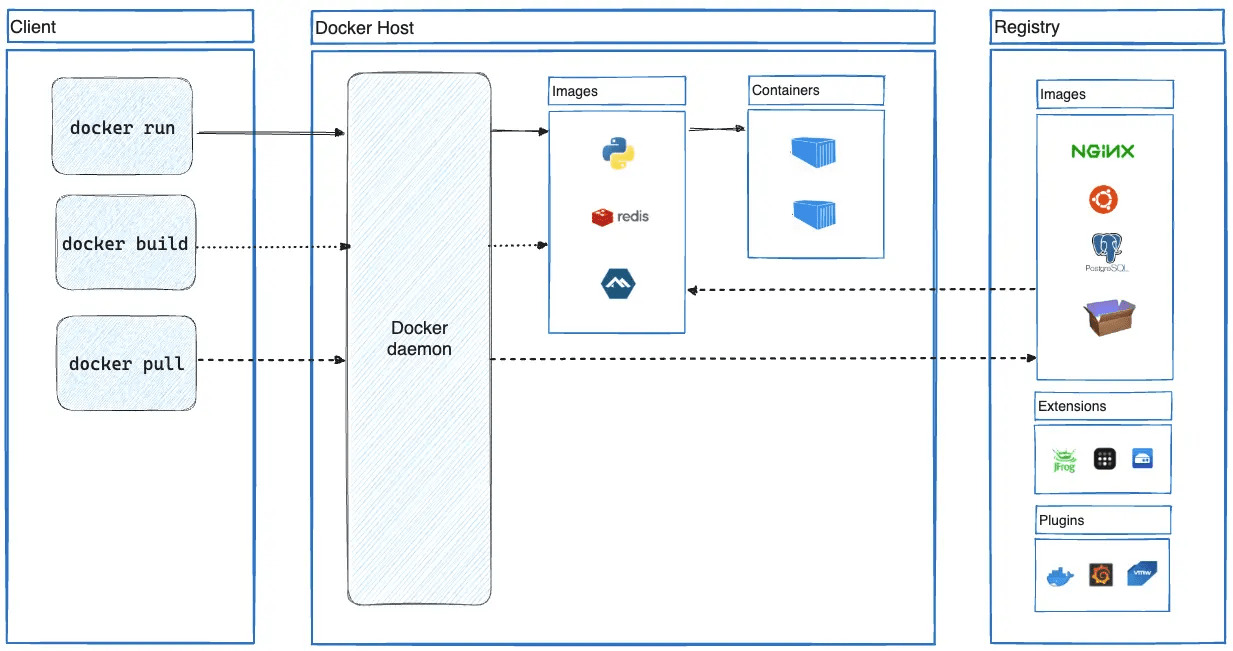
\includegraphics[width=12cm]{02_images/part_01/10_docker_architecture.png}
            \caption{Schéma de l'architecture Docker}
        \end{figure}

        L'adoption de Docker au sein de DASCH est donc stratégique. L'organisation a un Docker Hub dédié et cela permettra d'accélérer la livraison des applications et de les diffuser \footnote{Pour plus de détails sur les applications de \dsc sur Docker Hub, Voir \cite{daschswiss_dockerhub}.}.
        